\chapter{Dataset and Malware Detectors}

In order to successfully evaluate and analyze the malware detectors various experiments were performed using known Android malware. Once the android malware were finalized, the obfuscators were chosen to increase the difficulty of malware detection. A sampling was performed with a handful of malware. Using this sampling, the obfuscators to be applied were selected and then applied to a wider dataset. The results of this sampling are shown in Fig.\ref{sampling}.
 
 	 \vspace{3mm}
 	 \begin{center}
 	 	%\centering
 	 	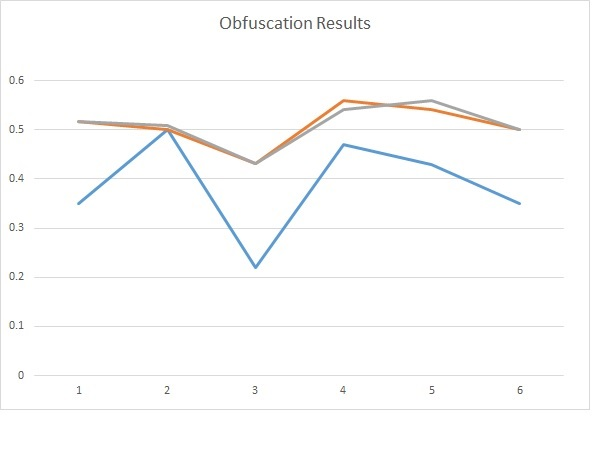
\includegraphics[width=0.8\textwidth]{sampling.jpg}
 	 	\captionof{figure}{Sampling Results}
 	 	\label{sampling}
 	 \end{center}
 	 \vspace{3mm}
 
 It can be seen from the results that only some obfuscators contribute effectively to hindering the detection ratio of malware obfuscators.
 
 \section{Dataset}
	 The Contagio dataset was used to perform the various experiments in this project \cite{contagio}. All the samples used for experimentation are malicious files. The files were classified as malicious by various means and the contagio data dump also certifies the files as being malware.
	 
	\subsection{Malware Files Selection}
		Known malicious files were used for performing the experiments in this project. The reason for using malware for the experiments was to understand how each obfuscator would help the malware in evading detection by malware detector. All the test samples were caught by at least one of the malware detectors and many of the samples were incorrectly classified as benign files, once the obfuscation was complete.

	\subsection{Other Datasets}
		Previously, experiments have been performed on malicious files belonging to other datasets. The results of a similar experiment performed on the Android
		Malware Genome Project \cite{zhou} are shown in Fig.\ref{genome}\cite{aamo}

		 \vspace{3mm}
		 \begin{center}
		 	%\centering
		 	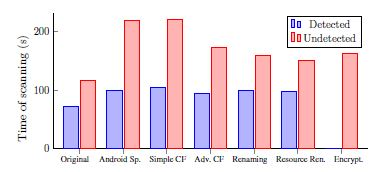
\includegraphics[width=0.8\textwidth]{genome.jpg}
		 	\captionof{figure}{Malware detector results for the Genome Project}
		 	\label{genome}
		\end{center}
		\vspace{3mm}
		
		
\section{Malware Detectors}
	A single malware detector is unlikely to give us a substantial result. This is because various malware detectors use different techniques for analyzing malware. If a single malware detector were to be used as a benchmark, then we would either get excellent detection scores or the malware detector would fail in a very poor way. To  overcome this shortcoming, a single obfuscated file is scanned by several malware detectors simultaneously.
	Instead of manually uploading the files to different malware detectors, we make use of VirusTotal \cite{virusTotal} and other similar virus scanning providers.